\hypertarget{hello-spring}{%
\section{\#3 Hello Spring}\label{hello-spring}}

\hypertarget{tutorial-build-a-spring-boot-application-using-intellij-idea}{%
\subsection{Tutorial: Build a spring boot application using intellij
idea}\label{tutorial-build-a-spring-boot-application-using-intellij-idea}}

\hypertarget{create-your-new-project-with-intellij}{%
\subsubsection{Create your new project with
intellij}\label{create-your-new-project-with-intellij}}

Open up IntelliJ and click on the Create New Project option.

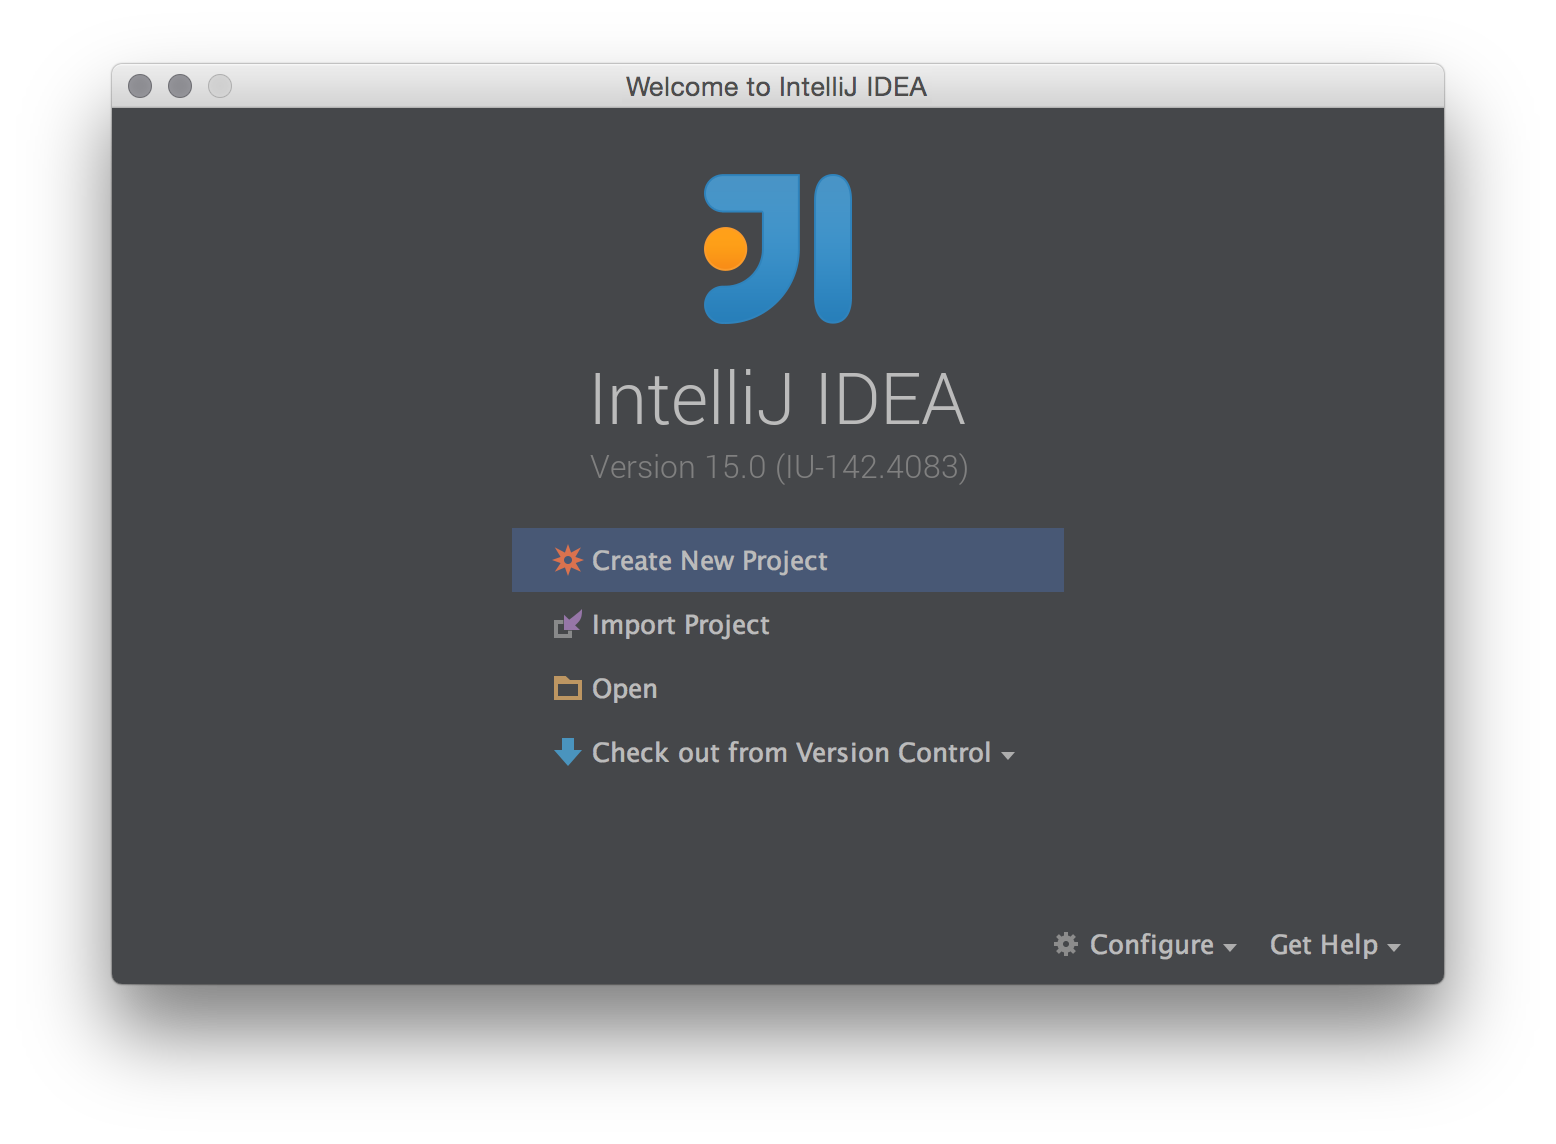
\includegraphics{rsc/1.png}

Next, select Spring Initializr from the project type in the left panel,
select your Project SDK and then click Next. The Initializr Service URL
should already be populated.

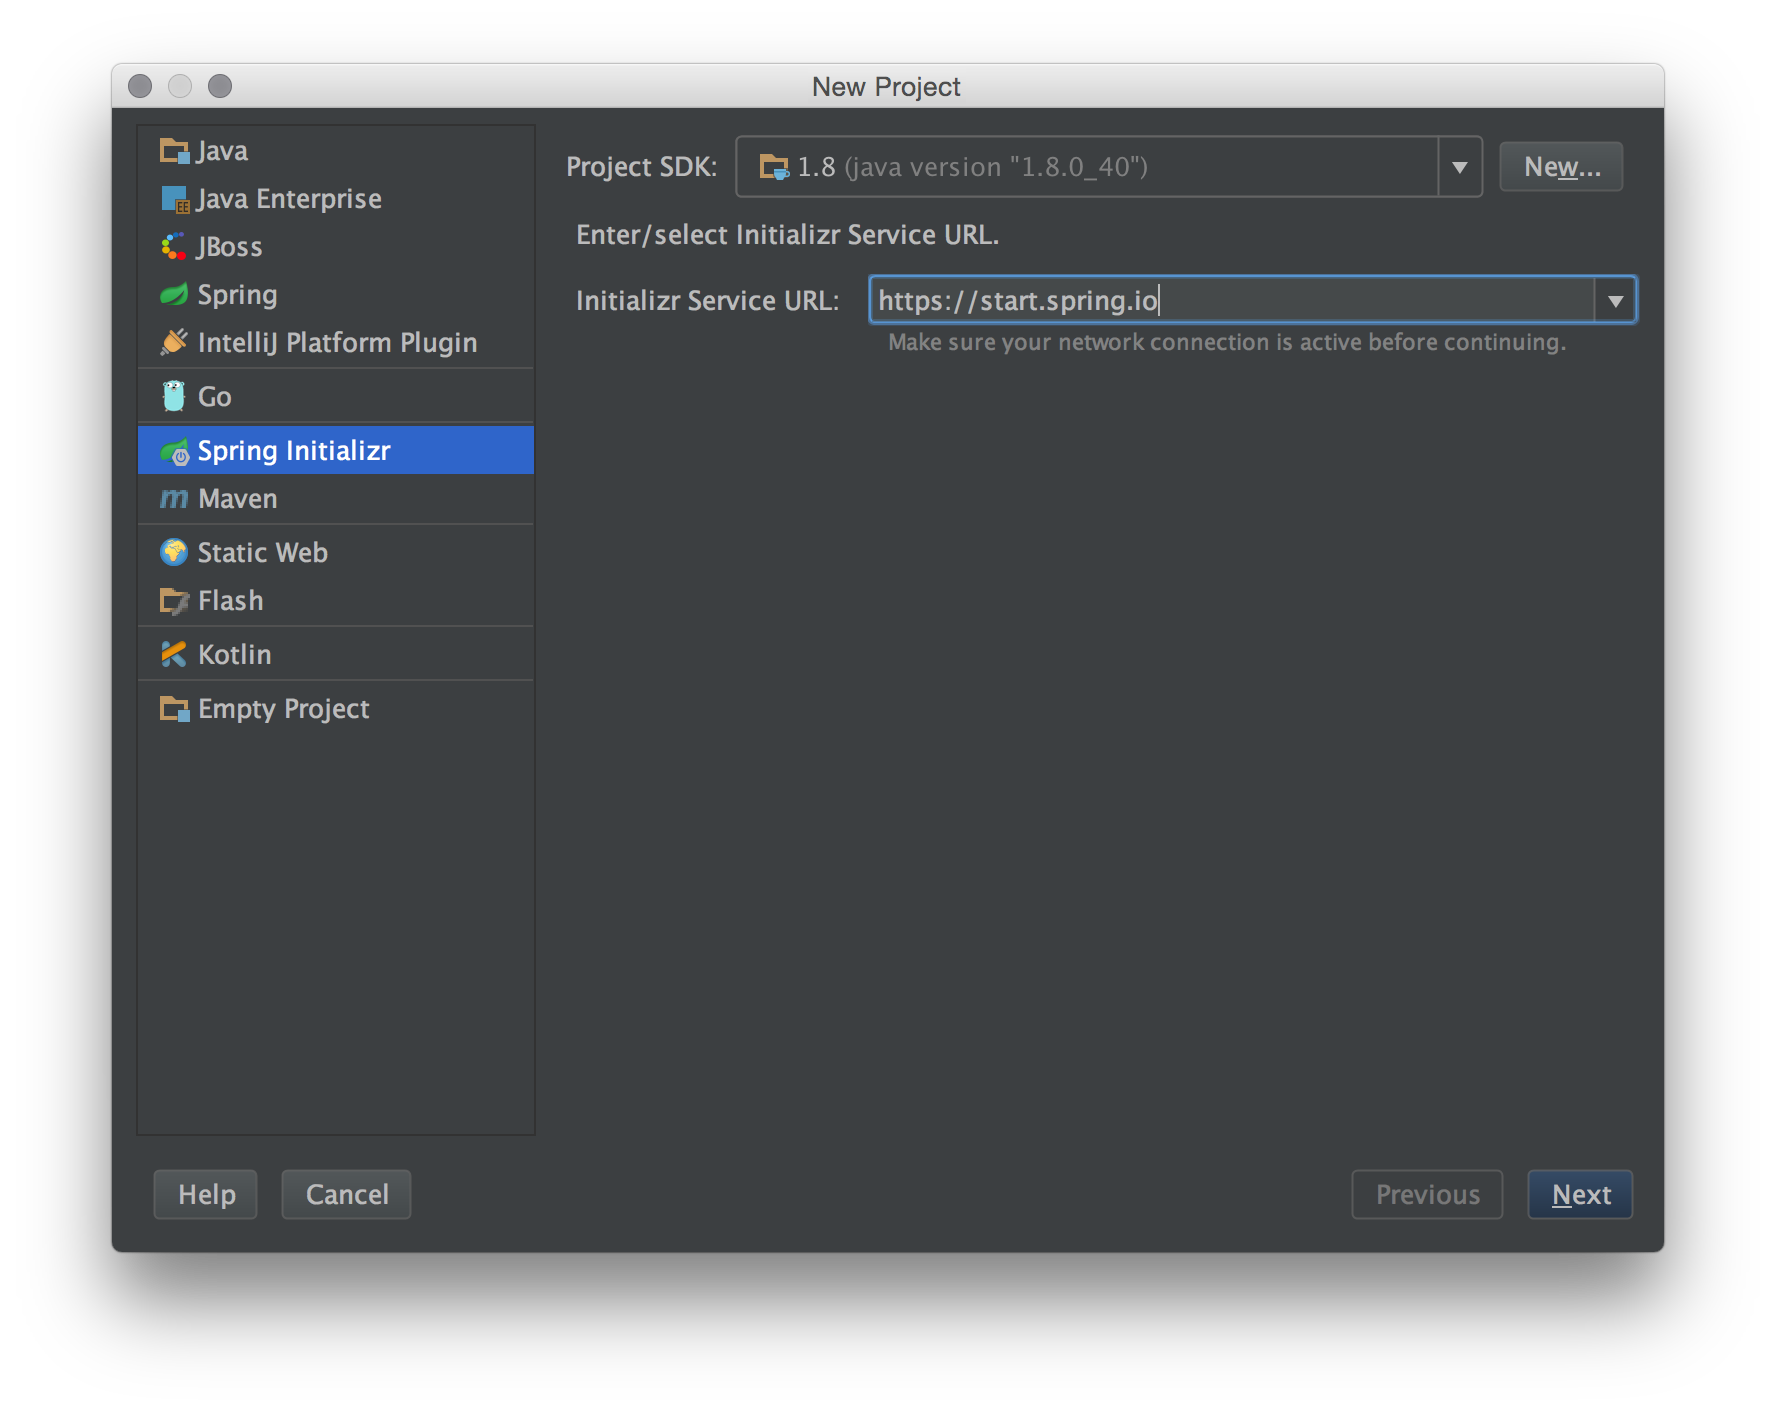
\includegraphics{rsc/2.png}

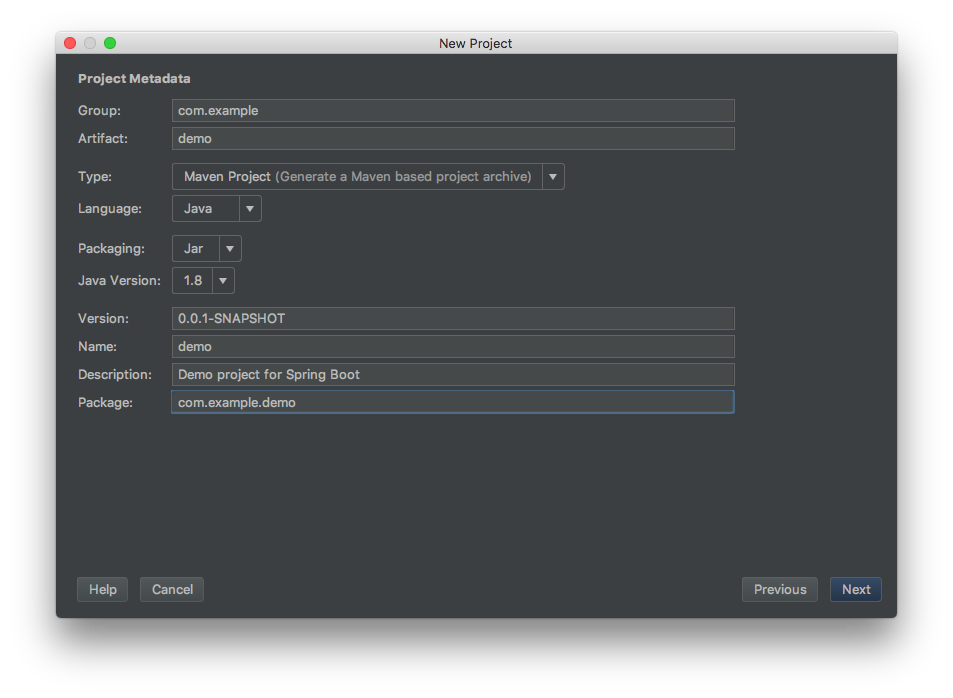
\includegraphics{rsc/3.png}

Next select any Spring Framework dependency your project will require.
here you should choose

\begin{itemize}
\tightlist
\item
  Web -\textgreater{} Web
\item
  Template Engines -\textgreater{} Thymeleaf
\end{itemize}

Click Next once you've selected all your dependencies.

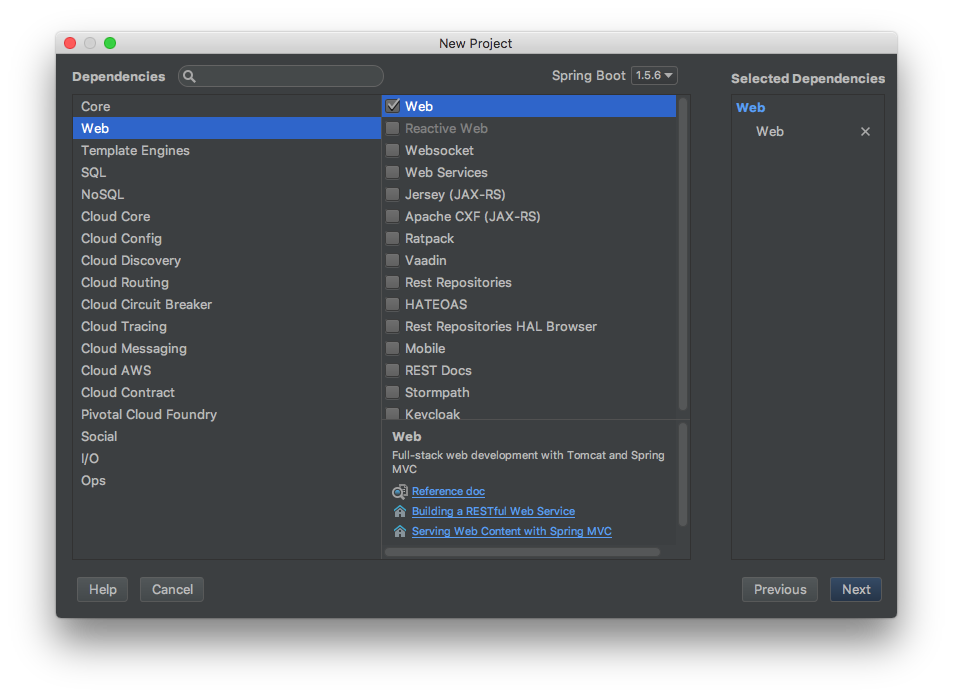
\includegraphics{rsc/4.png}

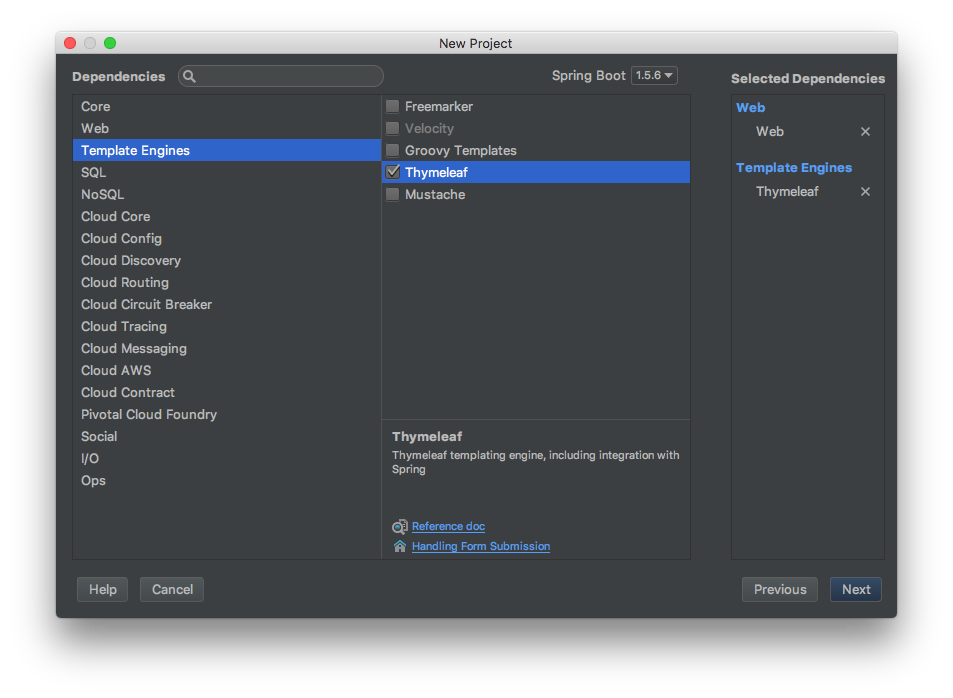
\includegraphics{rsc/5.png}

\emph{(heavily inspired by
https://patrickgrimard.io/2014/08/14/how-to-build-a-spring-boot-application-using-intellij-idea/)}

\_

© clbo@kea.dk

\_
